\section{Secondary market analysis}
\label{sec:methods}
Next, we seek to understand and quantify how names move between users. Our basic scenario is that Alice owns the name `d/example' and Bob would like to purchase it from her. We explore various ways this sale can occur and how these sales can be detected.

\subsection{Detecting atomic transfers}

\begin{figure*}
  \centering
  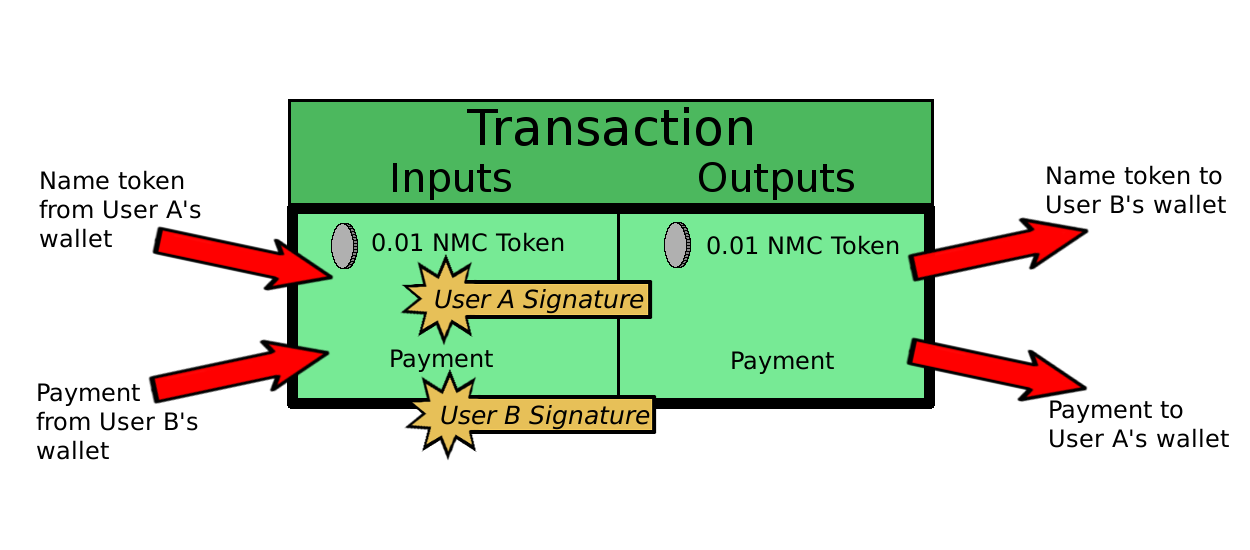
\includegraphics[width=0.9\textwidth]{figures/atomicTX}
  \caption{Functioning of atomic transactions}
  \label{fig:atomic}
\end{figure*}

The safest way to buy and sell Namecoin names is through the use of atomic transactions. This is an important technique in cryptocurrencies whereby two parties can exchange digital assets (such as a name in exchange for currency) without a trusted intermediary without either worrying that the other will abscond after receiving her half of the bargain. We show how these transactions work in Figure \ref{fig:atomic}. In an atomic transaction, Alice and Bob make their exchange in a single transaction. In the simplest form of atomic name transfer, Bob creates a transaction which transfers his payment to Alice and transfers `d/example' to him. He then sends this transaction to Alice, the owner of the name, who verifies it, signs, and broadcasts the transaction to the block chain. Both Alice and Bob's signatures are locked to the inputs and outputs of the transaction so neither input can be spent individually without the full transaction. This transaction provides cryptographic security to both Alice and Bob since either both the name and coins will be exchanged or nothing will. Although there is nothing inherently different looking about this transaction on the block chain, there are a few possible techniques to detect them by implementation quirks.

The Namecoin client is a fairly underdeveloped piece of software and thus there is no built-in method of performing atomic transactions. In order to accomplish this task, the Namecoin RPC client must be used from the command line. In order to simplify this task, a Namecoin developer created ANTPY \cite{antpy}, a piece of software to automate the creation of atomic transactions. This software has the quirk that the buyer's payment goes to the address that the seller held the name in. To find these transactions we queried the block chain for transactions with a {\tt NAME\_FIRSTUPDATE} or {\tt NAME\_UPDATE} input from the same address as a non name output. We then further reduced this set by eliminating transactions where the name stayed at the same address.

We searched throughout the history of the Namecoin block chain for transactions fitting this specification. Our query returned 13 transactions which we believe represent all transactions built by the ANTPY script. However this by no means represents all sales on the block chain. We next attempt to discover atomic transactions in a different way.

A implementation-agnostic method for detecting atomic name transfers is to find transactions that clearly use change addresses. This occurs when there are two non-name outputs in a transaction that has a name input. In this case the buyer did not want to pay all of his input to the seller and thus kept some for himself. This leaves the transaction with 3 outputs. Under normal circumstances, {\tt NAME\_UPDATE} transactions will only have two outputs, a name output and a change address. Thus every transaction with three outputs is very likely an atomic name transfer.

In the history of the Namecoin block chain, we found 6 transactions fitting this form. However 5 of the 6 were also detected by the previous (ANTPY) criterion.

The 14 atomic transactions which we detected are a lower bound for the number of name transfers. We are unable to query for all atomic transactions since if the buyer doesn't want any change from a purchase and the seller gives the buyer a new address to send payment to, the transaction is indistinguishable from a regular non-transferring name update.

\subsection{Deriving an upper bound on number of sales}

Following up on our lower bound from the previous section, we now derive an upper bound on the number of name sales using data from the block chain. Whereas atomic transactions, can (sometimes) be recognized simply from their contents, other name sale transactions are not recognizable. Here the payment could be a separate transaction or even made in a currency other than Namecoin. We would hope that we could detect changes in name ownership by looking at changes in which key owns a name. However, since the Namecoin client defaults to sending names to new addresses on update, there is no way to look at an update and tell whether or not a name is being transferred between owners.

In order to detect non-atomic transactions we must expand our view to the prior value of a name being updated. Certainly if the value does not change then the transaction is simply renewing the name, not transferring it. However considering all other transactions to be name transfers is far too conservative of a criterion. Users freely update the values of names whenever information in them becomes outdated.

\begin{figure}
  \centering
  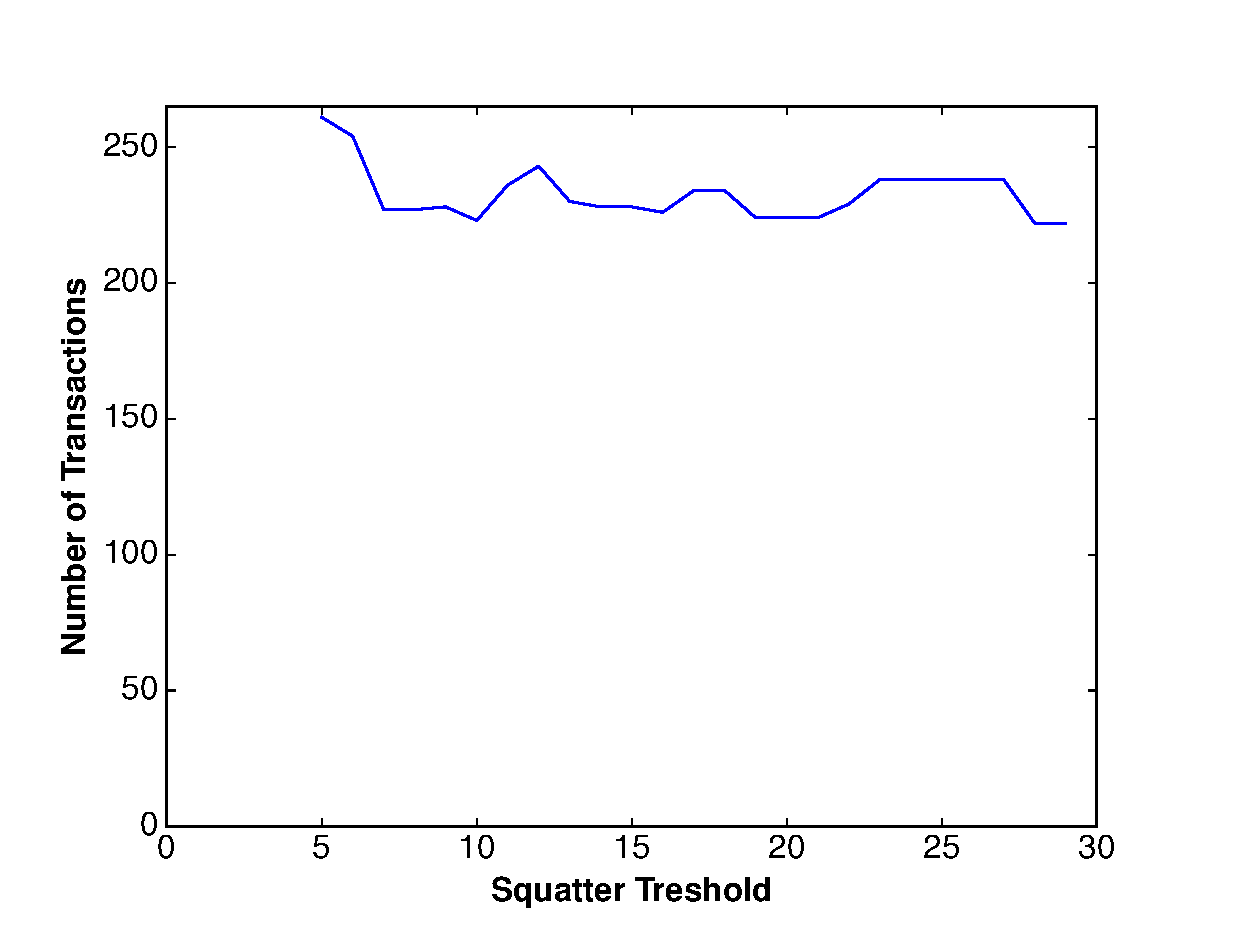
\includegraphics[width=0.9\columnwidth]{figures/transfers}
  \caption{Number of transfers detected based on squatting threshold. For each $n$ on the x-axis ($5 \leq n \leq 25$), we plot the number of squatter $\rightarrow$ non-squatter transactions detected if we characterize names whose values occur $n$ or more times as squatted.}
  \label{fig:percentSquatter}
\end{figure}

Although there doesn't seem to be a way to detect non-atomic name transfers generally, there is an important subclass of these transactions which can still be detected --- transfers from squatters to regular users. In the previous section we discussed our detection of squatters in the block chain which produces a list of values which with a high probability belong to squatters. Detecting transfers from squatters by finding names that change from one of these values to a value outside this set gives us a strategy to detect transfers.

We employ an additional criterion to eliminate false positives to tighten our upper bound. 
%Sometimes squatters update the value of their names, and thus a change from a squatter value may not represent the transfer of a name. To avoid picking up these updates as name transfers we restrict ourselves to selecting transactions that update the value of a name from a squatter value to a non-squatter value. 
If a name's value includes an info or email field and that stays the same in the updated value we can assume this is simply an update by the squatter. 

%Although this criterion is certainly not perfect, we believe that it has a fairly high success rate in revealing overall trends in name transfers.

Applying this analysis at various squatter threshold values, we see that the total number of squatter $\rightarrow$ non-squatter transactions detected holds at approximately 250 transactions. We emphasize that this value is likely an upper-bound since our criteria for reducing the number of transactions were quite conservative. 

To summarize, we would expect that given the high percentage of squatted .bit names, if there is a flourishing secondary market it would be dominated by sales from squatters to regular users. Yet we are able to upper bound the number of such transfers to about 250, a tiny fraction of the number of squatted names. Further, even though Namecoin supports a secure way to transfer names, we find strong evidence based on known tools supporting this functionality that its usage is very low.
